\documentclass{standalone}
\usepackage{tikz}
\begin{document}
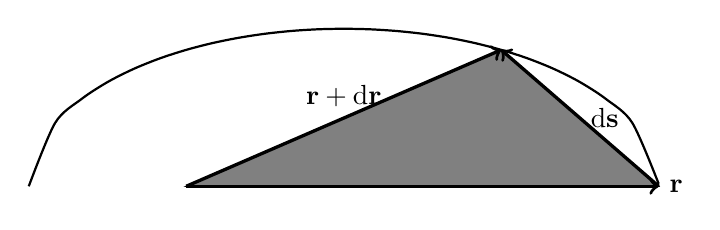
\begin{tikzpicture}[scale=2]
    \coordinate(O)at(-1,0);
    \draw[fill=gray](O)--(2,0)--(1,0.866)--cycle;
    \draw[-,thick]plot[smooth, domain=-2:2](\x,{(1-(\x)^2/4)^0.5});
    \draw[->,very thick](O)--(2,0)node[right]{$\mathbf{r}$};
    \draw[->,very thick](O)--(1,0.866)node[midway, above]{$\mathbf{r}+\mathrm{d}\mathbf{r}$};
    \draw[->,very thick](2,0)--(1,0.866)node[midway, right]{$\mathrm{d}\mathbf{s}$};
\end{tikzpicture}
\end{document}